% ============================================================
% CityBus - документација за проектна задача по Бази на податоци
% Компатибилно со Overleaf (pdfLaTeX)
% Слики за прикачување: stops.png, stop_lines.png, planner.png, live.png
% (од docs/screenshots/ во репозиториумот)
% ============================================================
\documentclass[11pt, a4paper]{article}

% - Кирилична поддршка -
% pdfLaTeX (стандардно во Overleaf): T2A фонтови; XeLaTeX/LuaLaTeX: истиот
% Computer Modern, во Unicode верзија (CMU), за да изгледа исто
\usepackage{iftex}
\ifPDFTeX
    \usepackage[T2A]{fontenc}
    \usepackage[utf8]{inputenc}
\else
    \usepackage{fontspec}
    \setmainfont{cmunrm.otf}[BoldFont=cmunbx.otf, ItalicFont=cmunti.otf,
                             BoldItalicFont=cmunbi.otf]
    \setsansfont{cmunss.otf}[BoldFont=cmunsx.otf, ItalicFont=cmunsi.otf,
                             BoldItalicFont=cmunso.otf]
    \setmonofont{cmuntt.otf}[ItalicFont=cmunit.otf]
\fi
% babel нема macedonian.ldf; македонскиот се вчитува од babel-mk.ini
\usepackage{babel}
\babelprovide[import, main]{macedonian}

% - Останати пакети -
\usepackage{geometry}
\geometry{a4paper, margin=2.2cm}
\usepackage{graphicx}
\graphicspath{{./}{docs/screenshots/}}
\usepackage{xcolor}
\usepackage{listings}
\usepackage{booktabs}
\usepackage{tabularx}
\usepackage{array}
\usepackage{caption}
\usepackage{subcaption}
\usepackage{enumitem}
\usepackage{titlesec}
\usepackage{float}
\usepackage{flafter}
\usepackage[section]{placeins}
\usepackage{tikz}
\usetikzlibrary{arrows.meta, positioning, shapes.multipart, calc, babel}
\usepackage[unicode]{hyperref}

\hypersetup{
    colorlinks=true,
    linkcolor=black,
    citecolor=black,
    urlcolor=blue,
    pdftitle={CityBus - документација за проектна задача},
    pdfauthor={Дамјан Зимбаков, Филип Карамачоски},
}

\titlespacing*{\section}{0pt}{2.6ex plus 1ex minus .2ex}{1.4ex plus .2ex}
\titlespacing*{\subsection}{0pt}{2.0ex plus 1ex minus .2ex}{1.0ex plus .2ex}
\captionsetup{font=small, labelfont=bf, skip=5pt}
\setlist{itemsep=1pt, topsep=3pt}
\setlength{\parskip}{4pt}
\setlength{\parindent}{0pt}
\setlength{\emergencystretch}{2em}

% страниците да се полнат до крај: без предност за прекин пред наслов
% (стандардно -300 остава празен простор на дното пред секое поглавје)
\makeatletter
\@secpenalty=0
\makeatother
% без прекин на страница по ред што завршува со цртичка (збор пре-/кинат меѓу страници)
\brokenpenalty=10000
% големите слики смеат да заземат поголем дел од страницата
\renewcommand{\topfraction}{0.85}
\renewcommand{\bottomfraction}{0.7}
\renewcommand{\textfraction}{0.1}
\renewcommand{\floatpagefraction}{0.75}

% долги идентификатори смеат да се прекршат по долната црта
\let\oldunderscore\_
\renewcommand{\_}{\oldunderscore\allowbreak}
\newcommand{\code}[1]{\texttt{#1}}
\newcommand{\ra}{$\rightarrow$}

% - Стил за приказ на SQL -
\lstdefinestyle{sql}{
    language=SQL,
    basicstyle=\ttfamily\footnotesize,
    keywordstyle=\color{blue!55!black}\bfseries,
    commentstyle=\color{black!50}\itshape,
    stringstyle=\color{green!40!black},
    backgroundcolor=\color{gray!8},
    frame=single,
    framerule=0pt,
    breaklines=true,
    showstringspaces=false,
    columns=fullflexible,
    keepspaces=true,
    aboveskip=6pt,
    belowskip=2pt,
    morekeywords={GENERATED, ALWAYS, IDENTITY, STORED, PARTITION, RANGE, OVER,
                  WINDOW, LEAD, EXTRACT, EPOCH, ANY, REFERENCES, CONSTRAINT,
                  CHECK, BETWEEN},
}
\lstset{style=sql}
% излез од EXPLAIN: само коментарите се обоени
\lstdefinelanguage{plan}{morecomment=[l]{--}}

% - Стилови за дијаграмите -
\colorlet{netc}{blue!14}
\colorlet{calc}{orange!22}
\colorlet{geoc}{green!16}
\colorlet{patc}{violet!14}
\colorlet{rtc}{red!13}
\tikzset{
    nohyph/.style={execute at begin node={\hyphenpenalty=10000\exhyphenpenalty=10000}},
    ent/.style={draw=black!60, rectangle split, rectangle split parts=2,
                rectangle split part fill={#1, white}, inner sep=1.7pt,
                text width=3.15cm, anchor=north west, nohyph,
                font=\ttfamily\fontsize{6.8}{8.1}\selectfont},
    wide/.style={text width=3.75cm},
    rel/.style={-{Latex[length=1.5mm, width=1.2mm]}, draw=black!55,
                line width=0.5pt, rounded corners=1.5pt},
    box/.style={draw=black!60, fill=#1, rounded corners=2pt, align=center,
                text width=3.25cm, minimum height=1.75cm, nohyph,
                font=\footnotesize, inner sep=3pt},
    flow/.style={{Latex[length=1.8mm]}-{Latex[length=1.8mm]}, draw=black!60,
                 line width=0.6pt},
}
\newcommand{\eh}[1]{{\fontsize{7.6}{8.8}\selectfont #1}}
\newcommand{\tg}[1]{\makebox[3.3em][l]{\rmfamily\fontsize{4.8}{5}\selectfont\bfseries #1}}
\newcommand{\PK}{\tg{\textcolor{red!60!black}{PK}}}
\newcommand{\FK}{\tg{\textcolor{blue!65!black}{FK}}}
\newcommand{\PF}{\tg{\textcolor{red!60!black}{PK}\,\textcolor{blue!65!black}{FK}}}
\newcommand{\UK}{\tg{\textcolor{green!40!black}{UK}}}
\newcommand{\NA}{\tg{}}
\newcommand{\ty}[1]{\hfill{\tiny\color{black!55}#1}}

\begin{document}

% ============================================================
% НАСЛОВНА СТРАНА
% ============================================================
\begin{titlepage}
    \centering
    \vspace*{1cm}

    {\large Универзитет „Св. Кирил и Методиј“ во Скопје \\[0.3cm]}
    {\large Факултет за информатички науки и компјутерско инженерство \\[0.15cm]}
    {\normalsize \href{https://finki.ukim.mk}{finki.ukim.mk} \\[2.2cm]}

    {\large Предмет: Бази на податоци \\[2cm]}

    {\Huge \textbf{CityBus} \\[0.4cm]}
    {\Large Систем за јавен градски превоз\\ заснован на GTFS база на податоци \\[0.5cm]}
    {\large Документација за проектна задача \\[3cm]}

    \begin{flushleft}
        \begin{tabular}{ll}
            \textbf{Автори:} & Дамјан Зимбаков \\
                             & Филип Карамачоски \\[0.3cm]
            \textbf{Ментор:} & проф. д-р Слободан Калајџиски \\
        \end{tabular}
    \end{flushleft}

    \vfill
    {\large Скопје, октомври 2026}
\end{titlepage}

\tableofcontents

\section*{Апстракт}

CityBus е систем за информации за јавниот градски автобуски превоз во Скопје, изграден околу релациона база на податоци во PostgreSQL 16 и PostGIS. Шемата го моделира стандардот GTFS во нормализирана форма, со просторни податоци, текстуално пребарување, планирање патувања со преседнувања и позиции на возилата во реално време. Над базата работат FastAPI backend и Flutter мобилна апликација. Документацијата ги опишува моделот на податоци и одлуките за индексирање и партиционирање, со мерења пред и по оптимизациите: на мрежа со 3,15 милиони \code{stop\_times} клучните барања се од 5,7 до околу 1\,000 пати побрзи, а еден ден телеметрија се брише со \code{DROP} на партиција за милисекунди, наместо со \code{DELETE} од стотици милисекунди што остава милион мртви редови.

% ============================================================
% 1. ВОВЕД
% ============================================================
\section{Вовед}

Патниците во јавниот превоз секојдневно ги поставуваат истите прашања: кои постојки се најблиску, кога поаѓа следниот автобус, како да стигнат од А до Б и каде е автобусот во моментов. Зад секој одговор стои барање (query) кон база со возни редови, географски податоци и податоци во реално време, па брзината на базата е брзина на апликацијата.

Стандардниот формат за возни редови е GTFS (General Transit Feed Specification)~\cite{gtfs}, кој го користат Google Maps и илјадници превозници. GTFS feed е збир од CSV датотеки (\code{stops.txt}, \code{trips.txt}, \code{stop\_times.txt}, \ldots) што сами по себе не се погодни за пребарување. CityBus ги претвора во нормализирана релациона шема и ги нуди преку REST API, WebSocket и мобилна апликација. Репозиториумот содржи синтетички, но реалистичен GTFS feed за Скопје: 5 линии, 30 постојки, 682 патувања и 6\,396 \code{stop\_times}, со работен и викенд возен ред, празничен исклучок и ноќно патување по полноќ.

\subsection{Цел на проектот}

Главниот резултат на проектот е базата на податоци; backend-от и апликацијата постојат за да покажат дека моделот работи од крај до крај. Целите се:
\begin{itemize}
    \item релационо моделирање на GTFS доменот со целосен интегритет (PK, FK, UNIQUE, CHECK);
    \item брзи одговори на просторните, текстуалните и временските прашања, со соодветен тип индекс за секое;
    \item планирање патувања со преседнувања, директно од податоците во \code{stop\_times};
    \item позиции на возила во реално време, без неограничен раст на податоците;
    \item мерливо докажување на придобивките од дизајнот (поглавје~\ref{sec:perf}).
\end{itemize}

\subsection{Линкови}

\begin{itemize}
    \item \textbf{Git репозиториум:} \url{https://github.com/zimbakovtech/citybus-app}
    \item \textbf{Веб-страница на проектот:} \url{https://zimbakovtech.github.io/citybus-app/}
\end{itemize}

% ============================================================
% 2. ТЕХНОЛОГИИ И АРХИТЕКТУРА
% ============================================================
\section{Технологии и архитектура}

\begin{table}[!htb]
\centering
\small
\begin{tabularx}{\textwidth}{@{}lX@{}}
\toprule
\textbf{Слој} & \textbf{Технологии} \\
\midrule
База на податоци & PostgreSQL 16, PostGIS 3.5, \code{pg\_trgm}, Alembic (миграции) \\
Backend & Python 3.11+, FastAPI, SQLAlchemy 2 (async) + asyncpg, GeoAlchemy2, Pydantic v2 \\
Мобилна апликација & Flutter, Dart, Riverpod 3, GoRouter, Dio, freezed, flutter\_map (OpenStreetMap) \\
Инфраструктура & Docker Compose, GitHub Actions (CI), GitHub Pages \\
\bottomrule
\end{tabularx}
\caption{Технологии на системот}
\end{table}

Системот има три дела (слика~\ref{fig:arch}). Увозникот го вчитува GTFS feed-от во базата. FastAPI backend-от е слоевит: \code{endpoints} (HTTP и валидација) \ra{} \code{services} (бизнис логика) \ra{} \code{repositories} (целиот SQL), а со базата комуницира преку асинхрониот SQLAlchemy 2. Flutter апликацијата ги прикажува податоците и прима ажурирања во реално време преку WebSocket.

\begin{figure}[!htb]
\centering
\begin{tikzpicture}[node distance=0.85cm]
    \node[box=geoc] (feed) {\textbf{GTFS feed}\\ \code{.txt} / \code{.zip}\\ \code{import\_gtfs.py}};
    \node[box=netc, right=of feed] (db) {\textbf{PostgreSQL 16}\\ \textbf{+ PostGIS 3.5}\\ GTFS шема, \code{pg\_trgm}};
    \node[box=patc, right=of db] (api) {\textbf{FastAPI backend}\\ REST + WebSocket\\ CSA, симулација};
    \node[box=calc, right=of api] (app) {\textbf{Flutter апликација}\\ Riverpod, Dio\\ flutter\_map (OSM)};
    \draw[-{Latex[length=1.8mm]}, draw=black!60, line width=0.6pt] (feed) -- node[above, font=\scriptsize] {увоз} (db);
    \draw[flow] (db) -- node[above, font=\scriptsize] {SQL} node[below, font=\scriptsize] {async} (api);
    \draw[flow] (api) -- node[above, font=\scriptsize] {REST} node[below, font=\scriptsize] {WS} (app);
\end{tikzpicture}
\caption{Архитектура на системот}
\label{fig:arch}
\end{figure}

% ============================================================
% 3. ИМПЛЕМЕНТАЦИЈА
% ============================================================
\section{Имплементација}

\subsection{Увоз на GTFS податоци}

Увозникот прво го валидира feed-от (задолжителни датотеки, единствени идентификатори, референци, формати) и секоја грешка ја пријавува со датотека, ред и поле. Потоа, во една трансакција, ги празни табелите со \code{TRUNCATE}, ги внесува родителите пред децата, ги пресликува GTFS идентификаторите во сурогат клучеви преку мапи во меморија, ги внесува \code{stop\_times} во серии од 5\,000 реда и на крајот ја склопува геометријата на секој shape. Повторното извршување го заменува feed-от, без дупликати.

\subsection{Backend и планер на патувања}

API-то (OpenAPI на \code{/docs}) нуди пребарување постојки и линии, најблиски постојки, поаѓања, постојки и GeoJSON полилинија на линија, планер и позиции на возилата; \code{WS /ws/realtime} праќа ажурирања на секои 2~s.

Планерот го користи Connection Scan Algorithm~\cite{csa}. Конекција е еден скок на едно патување меѓу две последователни постојки и се добива директно од \code{stop\_times} со window функцијата \code{LEAD}:

\begin{lstlisting}
SELECT st.stop_id AS dep_stop, LEAD(st.stop_id) OVER w AS arr_stop,
       EXTRACT(EPOCH FROM st.departure_time)::int AS dep_time,
       EXTRACT(EPOCH FROM LEAD(st.arrival_time) OVER w)::int AS arr_time,
       st.trip_id, t.route_id
FROM stop_times st JOIN trips t ON t.id = st.trip_id
WHERE t.service_id = ANY(:service_ids)
WINDOW w AS (PARTITION BY st.trip_id ORDER BY st.stop_sequence)
\end{lstlisting}

Конекциите се скенираат еднаш, по време на поаѓање. Ознаката на секоја постојка (време на пристигнување, број на возила) се споредува лексикографски, па меѓу еднакво брзи патувања победува она со помалку преседнувања; за преседнување се потребни најмалку 120~s, а се земаат предвид и патувањата од претходниот ден што продолжуваат по полноќ.

\subsection{Мобилна апликација}

Flutter апликацијата е организирана по функционалности (stops, routes, planner, live\_tracking), секоја со слоеви \code{data} (freezed модели, Dio, repository), \code{domain} (интерфејс) и \code{presentation} (Riverpod providers, страници). Навигацијата е со GoRouter, мапите со flutter\_map и OpenStreetMap, а маркерите на live мапата се поместуваат според пораките од WebSocket (слика~\ref{fig:app}).

\subsection{Тестирање и CI}

Backend-от има 53 pytest теста врз вистинска, мигрирана и наполнета база: API (вклучително поаѓања по полноќ и на празник), CSA и планер со познат одговор, валидација, realtime и WebSocket, и тестови на самата шема (генерирана геометрија, CHECK ограничувања, отсуство на редундантни индекси, партиции). Flutter апликацијата има 10 теста. GitHub Actions при секој pull request и push на \code{main} подига PostGIS service container, ги применува миграциите, го увезува seed feed-от и извршува ruff, black, pytest, \code{flutter analyze} и \code{flutter test}.

\begin{figure}[!tb]
\centering
\begin{subfigure}{0.19\textwidth}\centering
    \includegraphics[width=\linewidth]{stops.png}
    \caption{Постојки}
\end{subfigure}\hspace{0.03\textwidth}%
\begin{subfigure}{0.19\textwidth}\centering
    \includegraphics[width=\linewidth]{stop_lines.png}
    \caption{Поаѓања}
\end{subfigure}\hspace{0.03\textwidth}%
\begin{subfigure}{0.19\textwidth}\centering
    \includegraphics[width=\linewidth]{planner.png}
    \caption{Планер}
\end{subfigure}\hspace{0.03\textwidth}%
\begin{subfigure}{0.19\textwidth}\centering
    \includegraphics[width=\linewidth]{live.png}
    \caption{Live мапа}
\end{subfigure}
\caption{Изглед на мобилната апликација}
\label{fig:app}
\end{figure}

% ============================================================
% 4. БАЗА НА ПОДАТОЦИ
% ============================================================
\section{База на податоци}

\subsection{Модел на податоци}

Шемата има 14 табели (слика~\ref{fig:erd}) во пет целини: мрежа, календар, геометрија, шеми на линии и реално време. Најфина грануларност има \code{stop\_times}: еден ред е еден закажан настан, т.е. пристигнување и поаѓање на едно патување на една постојка. Сè друго ја опишува или агрегира: \code{trips} ги групира настаните на едно возење, \code{routes} ги групира патувањата во линија, календарот кажува во кои денови возат, а \code{stops} и \code{shapes} кажуваат каде.

\begin{figure}[!tb]
\centering
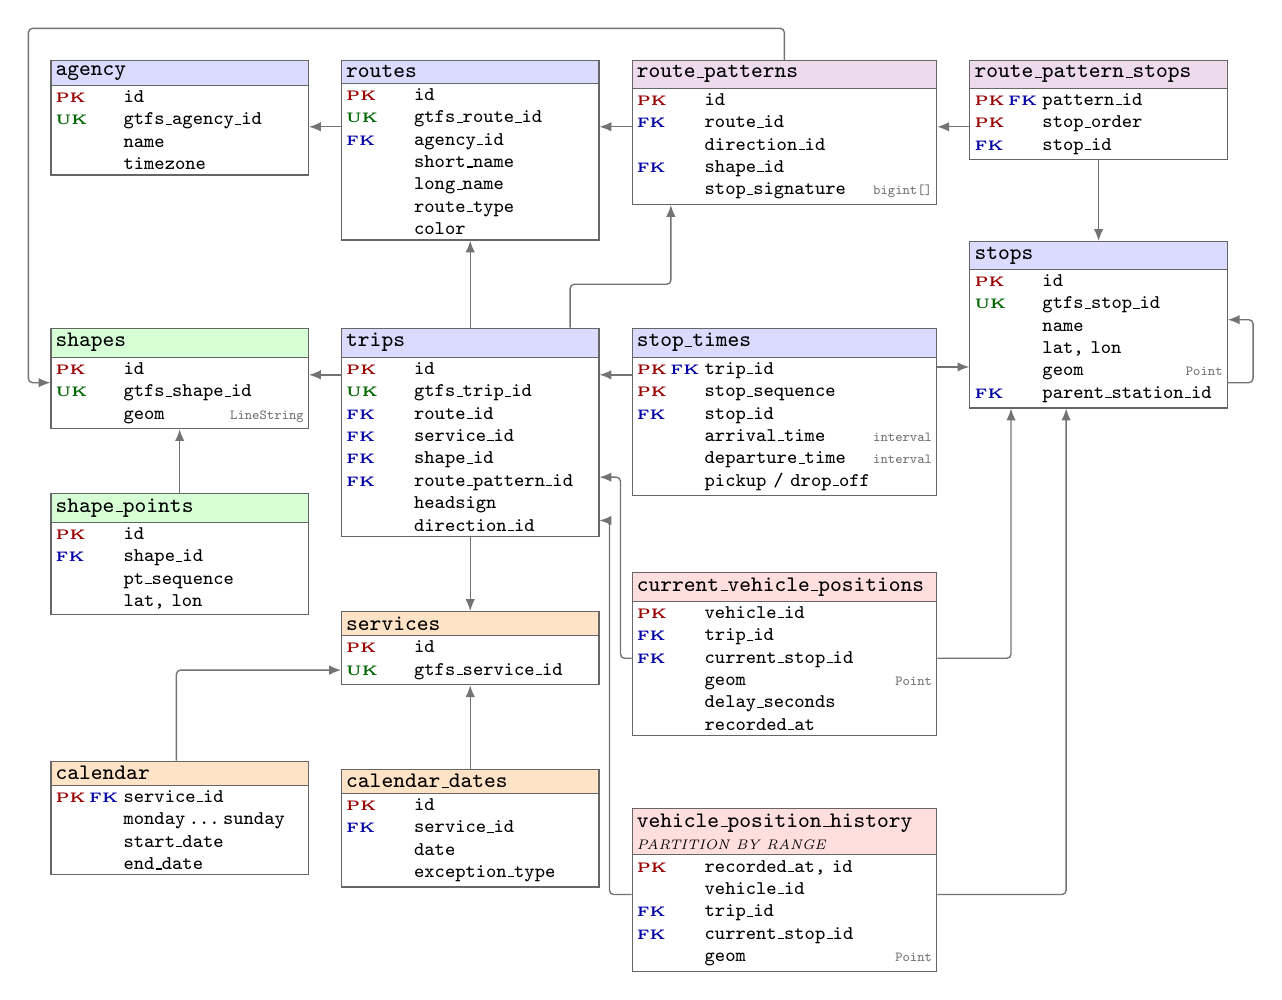
\begin{tikzpicture}[x=1cm, y=1cm]
    \let\_\oldunderscore
    % колони: 0, 3.69, 7.38 (поширока), 11.67
    \node[ent=netc] (agency) at (0,0) {\eh{agency}\nodepart{two}
        \PK id\\ \UK gtfs\_agency\_id\\ \NA name\\ \NA timezone};
    \node[ent=netc] (routes) at (3.69,0) {\eh{routes}\nodepart{two}
        \PK id\\ \UK gtfs\_route\_id\\ \FK agency\_id\\ \NA short\_name\\ \NA long\_name\\ \NA route\_type\\ \NA color};
    \node[ent=patc, wide] (rp) at (7.38,0) {\eh{route\_patterns}\nodepart{two}
        \PK id\\ \FK route\_id\\ \NA direction\_id\\ \FK shape\_id\\ \NA stop\_signature \ty{bigint[]}};
    \node[ent=patc] (rps) at (11.67,0) {\eh{route\_pattern\_stops}\nodepart{two}
        \PF pattern\_id\\ \PK stop\_order\\ \FK stop\_id};
    \node[ent=geoc] (shapes) at (0,-3.4) {\eh{shapes}\nodepart{two}
        \PK id\\ \UK gtfs\_shape\_id\\ \NA geom \ty{LineString}};
    \node[ent=netc] (trips) at (3.69,-3.4) {\eh{trips}\nodepart{two}
        \PK id\\ \UK gtfs\_trip\_id\\ \FK route\_id\\ \FK service\_id\\ \FK shape\_id\\ \FK route\_pattern\_id\\ \NA headsign\\ \NA direction\_id};
    \node[ent=netc, wide] (st) at (7.38,-3.4) {\eh{stop\_times}\nodepart{two}
        \PF trip\_id\\ \PK stop\_sequence\\ \FK stop\_id\\ \NA arrival\_time \ty{interval}\\ \NA departure\_time \ty{interval}\\ \NA pickup / drop\_off};
    \node[ent=netc] (stops) at (11.67,-2.3) {\eh{stops}\nodepart{two}
        \PK id\\ \UK gtfs\_stop\_id\\ \NA name\\ \NA lat, lon\\ \NA geom \ty{Point}\\ \FK parent\_station\_id};
    \node[ent=geoc] (sp) at (0,-5.5) {\eh{shape\_points}\nodepart{two}
        \PK id\\ \FK shape\_id\\ \NA pt\_sequence\\ \NA lat, lon};
    \node[ent=calc] (services) at (3.69,-7.0) {\eh{services}\nodepart{two}
        \PK id\\ \UK gtfs\_service\_id};
    \node[ent=rtc, wide] (cvp) at (7.38,-6.5) {\eh{current\_vehicle\_positions}\nodepart{two}
        \PK vehicle\_id\\ \FK trip\_id\\ \FK current\_stop\_id\\ \NA geom \ty{Point}\\ \NA delay\_seconds\\ \NA recorded\_at};
    \node[ent=calc] (calendar) at (0,-8.9) {\eh{calendar}\nodepart{two}
        \PF service\_id\\ \NA monday\,\ldots\,sunday\\ \NA start\_date\\ \NA end\_date};
    \node[ent=calc] (cd) at (3.69,-9.0) {\eh{calendar\_dates}\nodepart{two}
        \PK id\\ \FK service\_id\\ \NA date\\ \NA exception\_type};
    \node[ent=rtc, wide] (vph) at (7.38,-9.5) {\eh{vehicle\_position\_history}\\
        {\rmfamily\fontsize{5}{6}\selectfont\itshape PARTITION BY RANGE}\nodepart{two}
        \PK recorded\_at, id\\ \NA vehicle\_id\\ \FK trip\_id\\ \FK current\_stop\_id\\ \NA geom \ty{Point}};

    % релации: стрелката оди од FK кон PK што го референцира
    \draw[rel] (routes.west |- 0,-0.85) -- (agency.east |- 0,-0.85);
    \draw[rel] (rp.west |- 0,-0.85) -- (routes.east |- 0,-0.85);
    \draw[rel] (rps.west |- 0,-0.85) -- (rp.east |- 0,-0.85);
    \draw[rel] (rps.south) -- (rps.south |- stops.north);
    \draw[rel] (rp.north) -- ++(0,0.4) -| (-0.28,-4.1) -- (shapes.west |- 0,-4.1);
    \draw[rel] (trips.north) -- (trips.north |- routes.south);
    \draw[rel] (trips.north -| 6.6,0) -- (6.6,-2.85) -| (7.88,0 |- rp.south);
    \draw[rel] (trips.west |- 0,-4.0) -- (shapes.east |- 0,-4.0);
    \draw[rel] (st.west |- 0,-4.0) -- (trips.east |- 0,-4.0);
    \draw[rel] (st.east |- 0,-3.9) -- (stops.west |- 0,-3.9);
    \draw[rel] (sp.north) -- (sp.north |- shapes.south);
    \draw[rel] (trips.south) -- (trips.south |- services.north);
    \draw[rel] (1.6,0 |- calendar.north) |- (services.west |- 0,-7.75);
    \draw[rel] (cd.north) -- (cd.north |- services.south);
    \draw[rel] (cvp.west |- 0,-7.6) -- (7.24,-7.6) |- (trips.east |- 0,-5.3);
    \draw[rel] (vph.west |- 0,-10.6) -- (7.10,-10.6) |- (trips.east |- 0,-5.85);
    \draw[rel] (cvp.east |- 0,-7.6) -| (12.2,0 |- stops.south);
    \draw[rel] (vph.east |- 0,-10.6) -| (12.9,0 |- stops.south);
    \draw[rel] (stops.east |- 0,-4.1) -- ++(0.32,0) |- (stops.east |- 0,-3.3);
\end{tikzpicture}
\caption{ER дијаграм на базата. Стрелката оди од надворешниот клуч (FK) кон примарниот клуч (PK) што го референцира; UK е единствен природен клуч. Бојата ја означува целината: мрежа, календар, геометрија, шеми на линии и реално време.}
\label{fig:erd}
\end{figure}

\subsection{Клучни дизајн одлуки}

\begin{itemize}[leftmargin=*]
    \item \textbf{Сурогат клучеви, зачувани природни клучеви.} Секој ентитет има \code{bigint GENERATED ALWAYS AS IDENTITY} примарен клуч, а оригиналниот GTFS идентификатор е UNIQUE природен клуч. Надворешните клучеви ги референцираат сурогатите, па индексните записи и споредбите при join се 8-бајтни; GTFS идентификаторите и онака се единствени само во рамки на еден feed. Релациските табели имаат композитни клучеви, на пр. \code{(trip\_id, stop\_sequence)}.
    \item \textbf{\code{services} како посебен ентитет.} GTFS нема \code{services.txt}; \code{service\_id} се појавува во calendar, calendar\_dates и trips. Со посебна табела секој сервис е еден ред кон кој покажуваат сите три, а поддржани се и feed-ови што сервисите ги дефинираат само преку исклучоци.
    \item \textbf{\code{interval} наместо \code{time}.} Патување што поаѓа во 23:45 стигнува во „24:29:00“ и сè уште припаѓа на претходниот сервисен ден. Типот \code{time} го одбива ова (\code{date/time field value out of range}), па времињата се \code{interval} од полноќта на сервисниот ден, а поаѓањата и планерот ги разгледуваат и сервисите од претходниот ден.
    \item \textbf{Генерирана и изведена геометрија.} \code{stops.geom} е STORED генерирана колона од \code{lon}/\code{lat}, па координатите и геометријата не можат да се разминат. \code{shapes.geom} е LineString склопен еднаш при увоз со \code{ST\_MakeLine(\ldots{} ORDER BY pt\_sequence)}, па полилинијата за мапата е читање на еден ред.
    \item \textbf{Шеми на линии.} Патувањата со иста линија, насока, shape и подредени постојки делат шема, единствена преку \code{UNIQUE NULLS NOT DISTINCT (route\_id, direction\_id, shape\_id, stop\_signature)}. Разгранувањата и скратените варијанти се експлицитни, наместо скриени зад произволно „репрезентативно“ патување.
    \item \textbf{Интегритет во самата база.} NOT NULL каде што има смисла; CHECK за GTFS енумерациите и правилата (\code{exception\_type IN (1,2)}, опсег на координати, хексадецимална боја, \code{departure\_time >= arrival\_time}); намерна ON DELETE политика: CASCADE по хиерархијата route \ra{} trips \ra{} stop\_times, SET NULL за опционални референци и RESTRICT кога бришењето би оставило шема без постојки.
\end{itemize}

\begin{lstlisting}
CREATE TABLE stops (
    id    bigint GENERATED ALWAYS AS IDENTITY PRIMARY KEY,
    gtfs_stop_id text NOT NULL UNIQUE,
    lat   double precision NOT NULL CHECK (lat BETWEEN -90 AND 90),
    lon   double precision NOT NULL CHECK (lon BETWEEN -180 AND 180),
    geom  geometry(Point, 4326) GENERATED ALWAYS AS
              (ST_SetSRID(ST_MakePoint(lon, lat), 4326)) STORED NOT NULL,
    parent_station_id bigint REFERENCES stops(id) ON DELETE SET NULL,
    ...
);
\end{lstlisting}

\subsection{Стратегија на индексирање}

Секое често барање има индекс што одговара на неговиот предикат и редослед (табела~\ref{tab:idx}), а ниту еден индекс не е дупликат: миграцијата 0002 ги отстрани индексите што само ги повторуваа PK или UNIQUE ограничувања, а тест во CI проверува дека не постојат. B-tree не може да опслужи \code{ILIKE '\%\ldots\%'}, па за имињата се користи trigram GIN. Geometry GiST дава KNN редослед, но за филтер во метри е потребен посебен geography expression индекс (види~\ref{sec:results}).

\begin{table}[!htb]
\centering
\small
\let\_\oldunderscore
\begin{tabularx}{\textwidth}{@{}>{\raggedright\arraybackslash}p{7.6cm}lX@{}}
\toprule
\textbf{Индекс} & \textbf{Тип} & \textbf{Барање што го опслужува} \\
\midrule
\code{stops (geom)} & GiST & KNN \code{<->}: најблиски постојки, snap \\
\code{stops ((geom::geography))} & GiST & \code{ST\_DWithin} во метри \\
\code{stops (name)}, \code{routes (short\_name)}, \code{routes (long\_name)} & GIN & \code{ILIKE} со \code{gin\_trgm\_ops} \\
\code{stop\_times (stop\_id, departure\_time)} & B-tree & поаѓања; линии низ постојка \\
\code{stop\_times} PK \code{(trip\_id, stop\_sequence)} & B-tree & постојки на патување; \code{LEAD} \\
\code{calendar\_dates} UNIQUE \code{(service\_id, date)} & B-tree & активни сервиси за датум \\
\code{trips (route\_id, service\_id)} & B-tree & патувања на линија за датум \\
\code{vehicle\_position\_history (vehicle\_id, recorded\_at)} & B-tree & историја на возило \\
\bottomrule
\end{tabularx}
\caption{Главни индекси (останатите се B-tree врз надворешни клучеви)}
\label{tab:idx}
\end{table}

\subsection{Податоци во реално време}

GTFS-Realtime е заменет со симулација: позадинска задача на секои 2~s ја интерполира позицијата на секое возило меѓу двете тековни постојки според возниот ред. Првата верзија ги чуваше позициите во една append-only табела \code{vehicle\_positions}, која растеше без граница, а snapshot-от бараше \code{DISTINCT ON} врз неа. Миграцијата 0003 ја подели на две табели, кои симулаторот ги запишува во иста трансакција:
\begin{itemize}
    \item \code{current\_vehicle\_positions}: еден ред по возило, ажуриран со \code{INSERT \ldots{} ON CONFLICT (vehicle\_id) DO UPDATE}; live snapshot-от чита само неа;
    \item \code{vehicle\_position\_history}: append-only, \code{PARTITION BY RANGE (recorded\_at)}, по една партиција за секој UTC ден.
\end{itemize}
PL/pgSQL функцијата \code{maintain\_vehicle\_position\_partitions()} однапред креира партиции за 7 дена, со \code{DROP} ги отстранува партициите постари од 30 дена и ги брише застарените тековни состојби; \code{pg\_advisory\_xact\_lock} спречува две истовремени извршувања.

\subsection{Еволуција на шемата}

Шемата се менува само преку Alembic миграции: 0001 е непроменлива снимка на почетниот DDL, 0002 додава ограничувања, генерирана геометрија и geography индекс и ги брише редундантните индекси, 0003 ја воведува партиционираната историја, а 0004 ги изведува шемите на линии од постоечките патувања со \code{array\_agg}. Миграциите ги пренесуваат постоечките податоци и имаат \code{downgrade}, а 0002 и 0004 прекинуваат со \code{RAISE EXCEPTION} ако некој постоечки ред не ги исполнува новите правила.

% ============================================================
% 5. АНАЛИЗА НА ПЕРФОРМАНСИ
% ============================================================
\section{Анализа на перформанси: пред и по оптимизациите}
\label{sec:perf}

\subsection{Методологија}

Мерени се истите SQL барања што ги извршуваат repositories во backend-от, во две состојби. \emph{Пред}: без конкретниот индекс (\code{DROP INDEX} во трансакција што потоа се поништува со \code{ROLLBACK}), или со старата шема и стариот SQL од ревизиите 0001--0003. \emph{После}: тековната шема. Секое барање се извршува неколку пати за загревање и 21 пат мерено (5--11 пати за најбавните) со \code{EXPLAIN (ANALYZE, TIMING OFF)}; прикажана е медијаната на \emph{Execution Time}. Целото мерење е повторено три пати од почеток; медијаните на барањата во табела~\ref{tab:results} се разликуваат меѓу извршувањата најмногу 8\,\% (најчесто под 3\,\%).

Покрај seed feed-от, мерено е и на синтетичка мрежа генерирана детерминистички со SQL, околу 490 пати поголема по бројот на \code{stop\_times} (табела~\ref{tab:data}). Околина: PostgreSQL 16.9 и PostGIS 3.5.2 (имиџот \code{postgis/postgis:16-3.5}, ист како во Docker Compose и CI) во Docker на Apple Silicon (amd64 емулација), со стандардна меморија (\code{shared\_buffers} 128~MB, \code{work\_mem} 4~MB) и исклучен JIT. На природен хардвер апсолутните времиња би биле пониски; битни се односите. Скриптите за генерирање и мерење се во \code{database/benchmark/}.

\begin{table}[!htb]
\centering
\small
\begin{tabular}{@{}lrrrrr@{}}
\toprule
 & \textbf{stops} & \textbf{trips} & \textbf{stop\_times} & \textbf{shape\_points} & \textbf{телеметрија} \\
\midrule
Seed feed & 30 & 682 & 6\,396 & 170 & --- \\
Скалирана мрежа & 10\,000 & 114\,568 & 3\,153\,040 & 266\,000 & 5\,398\,525 \\
\bottomrule
\end{tabular}
\caption{Големина на податоците (скалирана мрежа: 500 линии, 1\,000 шеми, телеметрија од 25 возила на секои 2~s за 5 дена)}
\label{tab:data}
\end{table}

\subsection{Резултати}
\label{sec:results}

\begin{table}[!htb]
\centering
\small
\begin{tabularx}{\textwidth}{@{}Xrrr@{}}
\toprule
\textbf{Барање (скалирана мрежа)} & \textbf{Пред [ms]} & \textbf{После [ms]} & \textbf{Забрзување} \\
\midrule
Поаѓања од постојка, прозорец од 60~min & 78,18 & 0,072 & $\times$1086 \\
Најблиски постојки до 500~m (просек од 200 локации): & & & \\
\quad ревизија 0001 / без просторен индекс & 15,74 / 10,18 & 0,0209 & $\times$754 / $\times$488 \\
Snap на координата до најблиска постојка & 2,151 & 0,032 & $\times$67 \\
Пребарување постојки по име (број + страница) & 6,98 & 0,184 & $\times$38 \\
Live snapshot: една табела \ra{} тековна состојба & 0,834 & 0,046 & $\times$18 \\
Историја на возило за последниот час & 3,207 & 0,320 & $\times$10 \\
Постојки на линија: репрезентативно патување \ra{} шема & 0,439 & 0,048 & $\times$9,1 \\
Полилинија: склопување од 341 точка \ra{} LineString & 0,142 & 0,025 & $\times$5,7 \\
\bottomrule
\end{tabularx}
\caption{Медијана на времето на извршување пред и по оптимизацијата}
\label{tab:results}
\end{table}

\textbf{Поаѓања.} Најголем ефект има композитниот B-tree \code{(stop\_id, departure\_time)}. Без него, за да најде 32 кандидати (23 поаѓања по филтерот на сервис), базата ги чита и отфрла сите 3,15 милиони \code{stop\_times}; со него, Index Scan ги чита само тие 32 реда. Проверката „не е последна постојка“ се решава со Index Only Scan Backward по PK, без читање од табелата, а истиот индекс, преку водечката колона \code{stop\_id}, ги опслужува и линиите низ постојката.

\begin{lstlisting}[language=plan, basicstyle=\ttfamily\scriptsize]
-- before: no (stop_id, departure_time) index
Parallel Seq Scan on stop_times st (actual rows=11 loops=3)
  Filter: ((departure_time >= '08:00') AND (departure_time <= '09:00') AND (stop_id = 8))
  Rows Removed by Filter: 1051003
-- after: idx_stop_times_stop_dep
Index Scan using idx_stop_times_stop_dep on stop_times st (actual rows=32 loops=1)
  Index Cond: ((stop_id = 8) AND (departure_time >= '08:00') AND (departure_time <= '09:00'))
\end{lstlisting}

\textbf{Најблиски постојки.} Со индексите од ревизијата 0001 барањето беше \emph{побавно} отколку без индекс. Планерот бира KNN Index Scan по geometry GiST, а \code{ST\_DWithin} го применува како филтер. Во радиус од 500~m има просечно 4,2 постојки, а кај 199 од 200 локации помалку од \code{LIMIT 10}, па скенирањето не може да запре рано: за една вратена постојка отфрла 9\,999. Geography expression индексот од 0002 го претвора барањето во Bitmap Index Scan врз неколкуте кандидати во радиусот.

\textbf{Модел, не само индекси.} Дел од забрзувањата доаѓаат од моделот: шемите на линии го елиминираат агрегирањето на 3\,290 реда \code{stop\_times} при отворање на линија, зачуваната геометрија го елиминира склопувањето на полилинијата, а live snapshot-от чита 25 реда, колку и да има историја. На seed feed-от, пак, сите барања траат под 0,4~ms со и без индекси (за пребарувањето планерот дури избира Seq Scan), па придобивките се гледаат дури на големина на вистински град.

\subsection{Одржување и складирање}

Табела~\ref{tab:maint} ги споредува одржувањето и просторот. Партиционирањето само по себе не го забрзува бришењето (\code{DELETE} врз една партиција трае слично); добивката е што застарениот ден се отстранува како цела табела, без мртви редови и \code{VACUUM}. Бидејќи секој B-tree зафаќа простор и се ажурира при секое запишување, задржани се само индексите што ги користи некое барање.

\begin{table}[!htb]
\centering
\small
\let\_\oldunderscore
\begin{tabularx}{\textwidth}{@{}>{\raggedright\arraybackslash}X>{\raggedright\arraybackslash}p{5.0cm}>{\raggedright\arraybackslash}p{3.7cm}@{}}
\toprule
\textbf{Операција} & \textbf{Стара шема / алтернатива} & \textbf{Тековна шема} \\
\midrule
Бришење на 1 ден телеметрија (1\,080\,000 реда) & \code{DELETE} 310--450~ms; остануваат 1,08~M мртви редови, \code{VACUUM} уште 380--400~ms & \code{DROP} на партиција 0,5--1~ms (прв повик до 11~ms); веднаш ослободени 256~MB \\
PK индекс на \code{stop\_times} & 128~MB со GTFS текстуални клучеви (просечно 14,8~B) & 100~MB со \code{bigint} ($-22$\,\%) \\
Редундантен индекс \code{(trip\_id, stop\_sequence)} & +99~MB; увозот на \code{stop\_times} 15--25\,\% побавен & отстранет во 0002 \\
\bottomrule
\end{tabularx}
\caption{Одржување и простор (скалирана мрежа)}
\label{tab:maint}
\end{table}

% ============================================================
% 6. ЗАКЛУЧОК
% ============================================================
\section{Заклучок}

CityBus покажува дека добро моделирана релациона база може да го носи поголемиот дел од логиката на систем за јавен превоз. GTFS доменот е нормализиран, интегритетот е гарантиран со ограничувања во самата база, а секое клучно прашање има индекс што одговара на неговиот облик: GiST за просторот, trigram GIN за текстот и композитни B-tree индекси за возниот ред. Податоците во реално време се поделени на мала тековна табела и дневно партиционирана историја со автоматско задржување од 30 дена.

Мерењата покажуваат дека овие одлуки не се забележливи на мал примерок, но на мрежа со големина на град клучните барања ги забрзуваат од 5,7 до околу 1\,000 пати, а бришењето на стара телеметрија го претвораат од \code{DELETE} од стотици милисекунди со милион мртви редови во \code{DROP} што трае милисекунди. Следно тесно грло е планерот, кој при секое барање ја вчитува целата низа конекции за денот; понатамошна работа се кеширање на таа низа (или алгоритам како RAPTOR), увоз на вистински GTFS feed, вистински GTFS-Realtime извор и автентикација на корисници.

% ============================================================
% ЛИТЕРАТУРА
% ============================================================
\begin{thebibliography}{9}
\addcontentsline{toc}{section}{Литература}
\small
\bibitem{gtfs} GTFS Schedule Reference. \url{https://gtfs.org/documentation/schedule/reference/}
\bibitem{pg} PostgreSQL 16 Documentation: Indexes, Table Partitioning, Using EXPLAIN. \url{https://www.postgresql.org/docs/16/}
\bibitem{postgis} PostGIS 3.5 Manual. \url{https://postgis.net/docs/}
\bibitem{trgm} PostgreSQL 16 Documentation: pg\_trgm. \url{https://www.postgresql.org/docs/16/pgtrgm.html}
\bibitem{csa} J. Dibbelt, T. Pajor, B. Strasser, D. Wagner. \emph{Intriguingly Simple and Fast Transit Routing}. Experimental Algorithms (SEA 2013), LNCS 7933, Springer, 2013, стр. 43--54.
\end{thebibliography}

\end{document}
